\documentclass[conference]{IEEEtran}
\IEEEoverridecommandlockouts
% The preceding line is only needed to identify funding in the first footnote. If that is unneeded, please comment it out.
\usepackage[portuguese]{babel} % for dates and expressions as “table of contents”, “chapter” or “appendix” translated
\usepackage[utf8]{inputenc} % for keyboard pt-br
\usepackage{multirow}
\usepackage{cite}
\usepackage{amsmath,amssymb,amsfonts}
\usepackage[portuguese, ruled, linesnumbered]{algorithm2e}
\usepackage{graphicx}
\usepackage{textcomp}
\usepackage{xcolor}
\def\BibTeX{{\rm B\kern-.05em{\sc i\kern-.025em b}\kern-.08em
    T\kern-.1667em\lower.7ex\hbox{E}\kern-.125emX}}
\begin{document}

\title{REST vs. GraphQL: Análise de desempenho com Python, PostgreSQL e Endereços Brasileiros\\
}

\author{\IEEEauthorblockN{Patrick Silva Ferraz}
\IEEEauthorblockA{\textit{Dep. de Ciência da Computação} \\
\textit{Universidade Federal da Bahia}\\
Salvador, Brasil \\
patrick.ferraz@outlook.com}
\and
\IEEEauthorblockN{Rita de Cássia Novaes Barretto, MSc}
\IEEEauthorblockA{\textit{Dep. de Ciência da Computação} \\
\textit{Universidade Federal da Bahia}\\
Salvador, Brasil \\
rb.dccufba@gmail.com}
\and
\IEEEauthorblockN{Cássio Vinícius Serafim Prazeres, PhD}
\IEEEauthorblockA{\textit{Dep. de Ciência da Computação} \\
\textit{Universidade Federal da Bahia}\\
Salvador, Brasil \\
cprazeres@gmail.com}
}

\maketitle

\begin{abstract}
A busca de endereços brasileiros em mapas é de fundamental importância para diversas atividades. Permite que, ao fornecer apenas o nome do logradouro, diversos endereços sejam localizados em diferentes áreas do país. Prover funcionalidades de software por meio de RESTful APIs é uma prática comum em aplicações geoespaciais. Com o intuito de acessar endereços na base do CEP Aberto, foram desenvolvidas duas APIs, sendo uma REST e outra GraphQL. Assim, tornou-se inevitável a comparação entre elas, em termos de eficiência de desempenho, seguindo as métricas ISO/IEC 9126 e 25010. Este trabalho pretende mostrar se a API GraphQL é tão eficiente quanto a API REST, a qual vem sendo amplamente utilizada. Esta resposta pode influenciar na elaboração de melhores projetos de arquitetura de Tecnologia da Informação - TI, que venham a ser implementados com a linguagem de programação Python e o banco de dados PostgreSQL.
\end{abstract}

\begin{IEEEkeywords}
rest, graphql, api, web service, python, postgresql, cep aberto
\end{IEEEkeywords}

\section{Introdução}
\label{sec:introducao}

No Brasil, são muitos os problemas relativos a cadastros, especificamente à falta de completeza e confiabilidade dos dados administrativos. Nas três esferas de governo, a saber: federal, estadual e municipal, quando existem processos de negócio de registros de dados, em geral, são falhos ou não são seguidos pelos usuários como deveriam, ocasionando erros de preenchimento. Por outro lado, não existe boa interação humano-computador, de forma que a inserção dos dados nos sistemas de informação também deixa a desejar. Assim, os cadastros destes sistemas apresentam um alto percentual de endereços indevidos, ilegíveis ou simplesmente inexistentes. Em paralelo a isso, métodos para determinar uma localização em um mapa digital ou encontrar o caminho ideal para chegar até lá estão se tornando cada vez mais relevantes para a vida cotidiana e nas pesquisas acadêmicas.
		
Endereços existem para facilitar a localização de uma unidade imobiliária. Excetuando-se as capitais Brasília/DF e Palmas/TO, as quais são planejadas, via de regra, os endereços brasileiros consistem dos seguintes atributos: tipo de logradouro; nome do logradouro; número; complemento; bairro; localidade; município; estado e CEP. Diante da baixa qualidade dos valores destes atributos nos cadastros, a identificação do ponto exato do imóvel, torna-se muito mais difícil e onerosa. A ideia de simplificar a busca, utilizando somente o nome do logradouro como parâmetro em pesquisa numa base de CEPs colaborativa, pode facilitar a localização de diversos endereços em diferentes regiões do país.
	
De acordo com o contexto, este trabalho pretende saber se, para os dados administrativos com baixa qualidade, acessar um lote de endereços, utilizando-se uma  \textit{application programming interface} - API GraphQL é tão eficiente quanto o uso da API \textit{Representational State Transfer} - REST, visando à avaliação da latência e \textit{overfechting}?

A hipótese é que a API GraphQL será mais eficiente com relação ao \textit{overfechting} e possivelmente à latência, uma vez que o acesso retornará um lote de endereços, em vez de um único. 

\subsection{Escopo e estrutura do artigo}
O escopo deste estudo consiste do levantamento de requisitos, desenvolvimento e teste de uma API REST, baseada em HTTP, e outra API GraphQL, para acesso aos dados do projeto CEP Aberto \cite{CEPAberto:2019}. Uma comparação da eficiência de desempenho de ambas, seguindo as métricas ISO 9126 e ISO 25010, faz-se necessária para subsidiar a tomada de decisão quanto a projetos arquiteturais que venham a ser implementados com a linguagem de programação Python e o banco de dados PostgreSQL, bem como envolvam acesso a endereços em bases de dados georreferenciados.
	
O conteúdo do artigo está organizado em cinco seções. A seção \ref{sec:introducao} é a introdução, que destaca o escopo e a estrutura do artigo. A seção \ref{sec:ref_teorico} é o referencial teórico, ressaltando API, REST, GraphQL, normas e padrões da ISO/IEC, assim como as métricas para comparação. A seção \ref{sec:arquitetura} apresenta as arquiteturas desenhadas. A seção \ref{sec:analise_desempenho} demonstra a análise de desempenho, detalhando o pré-processamento, a aplicação e comparação dos métodos, assim como os resultados. A Seção \ref{sec:discussao} resume as discussões e aponta desdobramentos futuros.

\section{Referencial teórico}
\label{sec:ref_teorico}

\subsection{API}
Durante anos, diversas alternativas de software surgiram para facilitar a comunicação entre aplicações ou entre um usuário e uma  aplicação. À estas alternativas, foi dado o nome de Application Programming Interface - API.

Em verdade, uma API trata-se de rotinas desenvolvidas e padrões estabelecidos e documentados por uma aplicação, para que usuários ou outras aplicações utilizem as funcionalidades daquela, sem precisar conhecer detalhes do software. Assim, as APIs implementam interoperabilidade entre aplicações.

Um exemplo é o Google Maps \cite{GoogleMaps:2019} que é um Geographical Information System - GIS baseado em nuvem e que combina mapas, imagens de satélite e informações geoespaciais, provendo APIs para que usuários ou outras aplicações possam ter acesso ao seu conteúdo.\cite{nourjou:2016}

\subsection{REST}

De acordo com \cite{jiang:2018}, fornecer funcionalidade de software por meio de APIs é uma prática comum em aplicativos geoespaciais. Por meio de um serviço da Web leve e escalável, clientes podem acessar ou processar dados geoespaciais sem complicação. Entre os provedores de API de geocodificação atuais, estão: a API de geocodificação do ArcGIS \cite{ArcGISAPIREST:2019}; a API de geocodificação aberta do MapQuest \cite{MapQuestAPIREST:2019} e a API de geocodificação what3words - w3w \cite{w3wAPI:2019}.

Neste trabalho, para implementar a busca de lotes de endereços foi projetada uma API para usar dados da plataforma CEP Aberto \cite{CEPAberto:2019}. \textit{Representational State Transfer} - REST é um estilo arquitetônico de rede que é aplicado a projetos de API para serviços da Web \cite{masse2011rest}. Uma API em conformidade com a mencionada arquitetura é considerada RESTful.  Um cliente pode obter dados do serviço da Web, enviando uma solicitação para um Uniform Resource Locator - URL específico por meio de uma API REST, que utiliza o Hyper Text Transfer Protocol - HTTP. Segundo \cite{ritsila2018graphql}, este tipo de API apresenta problemas, principalmente com o surgimento de aplicativos para dispositivos móveis, pelo fato das consultas REST exigirem muitos HTTP \textit{endpoints}, os quais retornam estruturas de dados fixas, podendo resultar em excesso de dados.

\subsection{GraphQL}
Diante desse cenário que apontava para a obsolescência da RESTful API, em 2012, o Facebook construiu a GraphQL para seus aplicativos Web e móveis. Em 2015, tornou-a pública. As necessidades de mais flexibilidade e eficiência na comunicação entre cliente e servidor foram decisivas para o planejamento e execução do projeto. De acordo com \cite{ritsila2018graphql}, a GraphQL possui um \textit{endpoint}  "inteligente"  que pode executar operações complexas e retornar apenas os dados que o cliente precisa. A forma da resposta corresponde à forma da consulta. Portanto, a GraphQL minimiza a quantidade de dados transferidos e permite uma fácil evolução das aplicações.

\subsection{ISO/IEC 9126 e 25010}
Visando à alta qualidade, a comparação das mencionadas APIs baseou-se nos padrões internacionais das entidades: International Organization for Standardization – ISO e International Electrotechnical Commission – IEC. Especificamente, nas métricas ditadas pelas ISO/IEC 9126 \cite{iso9126} e ISO/IEC 25010 \cite{iso25010}, as quais são voltadas para qualidade de software.

De acordo com \cite{iso9126}, as métricas de eficiência listadas na ISO/IEC TR 9126-3: 2003 não pretendem ser um conjunto exaustivo. Avaliadores podem selecioná-las para avaliar produtos de software, medir aspectos de qualidade e outros propósitos. Uma vez que, a ISO / IEC TR 9126-3: 2003 não atribui intervalos de valores dessas métricas a níveis nominais ou a graus de conformidade, eles foram definidos na Subseção \ref{subsec:metricas}, para atender a essa comparação entre APIs.

\subsection{Métricas para comparação}
\label{subsec:metricas}

É possível avaliar um sistema computacional com a utilização de diversos parâmetros, que tem como propósito computar o uso de recursos como a memória, o processamento e até a taxa transmissão em rede. Alguns destes estão relacionados com o cálculo da latência e \textit{overfetching}, respectivamente, o tempo que leva uma chamada atômica na API e o fato do cliente baixar mais informações do que é realmente necessário no aplicativo.

Segundo \cite{graphql:2019}, o que evidencia a superioridade da GraphQL em relação a aplicações com a arquitetura REST, refere-se principalmente ao \textit{overfetching}. Isto é o que este trabalho busca comprovar.

Em sistemas REST, \textit{endpoints} são utilizados para obter uma certa informação da API. Eles possuem o corpo de retorno padrão, muitas vezes sendo a estrutura completa da entidade do banco de dados. GraphQL pode ou não possuir uma estrutura semelhante, a grande diferença está na flexibilidade em relação ao que se quer obter, ou seja, é possível escolher os campos específicos que se pretende obter da entidade, evitando assim o \textit{overfetching}. \cite{graphql:2019} afirma que, com a utilização do GraphQL "Você pede o que quer e obtém resultados previsíveis".

Por fim, é possível utilizar os resultados obtidos para avaliar a latência. Embora a API GraphQL aparente retornar o resultado com atraso em relação à API REST, o corpo do conteúdo da GraphQL pode ser menor. Assim, pacotes menores serão transmitidos na rede, diminuindo a latência. 

Abaixo, segue uma descrição das métricas adaptadas de \cite{kleiman:2018}:

\begin{enumerate}
\item Categoria - Comportamento em relação ao tempo.
\subsubsection{Nome da Métrica - Latência}\label{BB}
\begin{enumerate}
\item Propósito da Métrica - Determinar o tempo para realizar uma chamada atômica na API;
\item Método da Métrica - Avaliar a velocidade de resposta a chamadas para backend para operações atômicas. Será medido o tempo completo desde que se realize a chamada a API até que se retorne a resposta desejada;
\item Fórmula:
\begin{equation}
x = tempo\ calculado\label{eq:latencia}
\end{equation}
\item Interpretação - Quanto menor o valor obtido, melhor;
\item Tipo de Medida: $x = ms$;
\item Origem da Medida - Tempo esperado de uma chamada atômica para o backend.
\end{enumerate}
\item Categoria - Utilização de recursos.
\subsubsection{Nome da Métrica - \textit{Overfechting}}\label{CC}
\begin{enumerate}
\item Propósito da Métrica - Determinar a porcentagem de informações supérfluas, em média, num conjunto de chamadas;
\item Método da Métrica - Estimar a eficiência das respostas recebidas por meio da API;
\item Fórmula:
\begin{equation}
x = total\ de\ bytes - bytes\ usados\label{eq:over}
\end{equation}
\item Interpretação - Quanto menor o valor, melhor;
\item Tipo de Medida: $x = bytes$;
\item Origem da Medida - Número de bytes retornados pela API e número de bytes que foram usados.
\end{enumerate}
% \subsubsection{Nome da Métrica - \textit{Underfechting}}\label{DD}
% \begin{enumerate}
% \item Propósito da Métrica - Determinar o número de chamadas, em média, necessárias para obter as informações desejadas;
% \item Método da Métrica - Estimar a eficiência das respostas recebidas por meio da API.;
% \item Fórmula - $X = quantidade de chamadas realizadas.$;
% \item Interpretação - Quanto menor o número de chamadas, melhor;
% \item Tipo de Medida - $X = chamadas$;
% \item Origem da Medida - Número de chamadas feitas pelo frontend.
% \end{enumerate}
\end{enumerate}

\section{Arquitetura}
\label{sec:arquitetura}

Dois modelos arquiteturais foram elaborados para o desenvolvimento das APIs (REST e GraphQL). O padrão Model View Controller - MVC foi adotado, visando à criação de certa semelhança entre as arquiteturas.

\begin{figure}[htbp]
\centerline{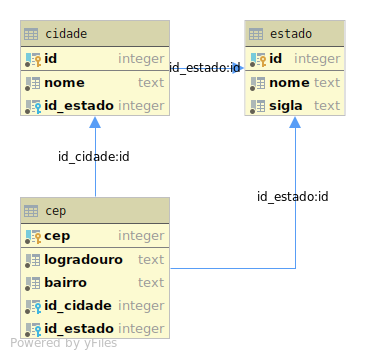
\includegraphics[scale=0.45]{imgs/database.png}}
\caption{Diagrama de entidade e relacionamento do banco de dados.}
\label{fig:der_database}
\end{figure}

As arquiteturas contam com três entidades: \textit{state} (estado), \textit{city} (cidade), \textit{place} (logradouro), modelados conforme a Figura \ref{fig:der_database}, onde \textit{state} e \textit{city} possuem uma \textit{id} como chave primária e campos referentes aos respectivos nomes, siglas e relações entre si, enquanto que \textit{place} possui o CEP como chave primária, \textit{ids} para referenciar o estado e a cidade ao qual pertence, nome do bairro e nome do logradouro.

\begin{figure}[htbp]
\centerline{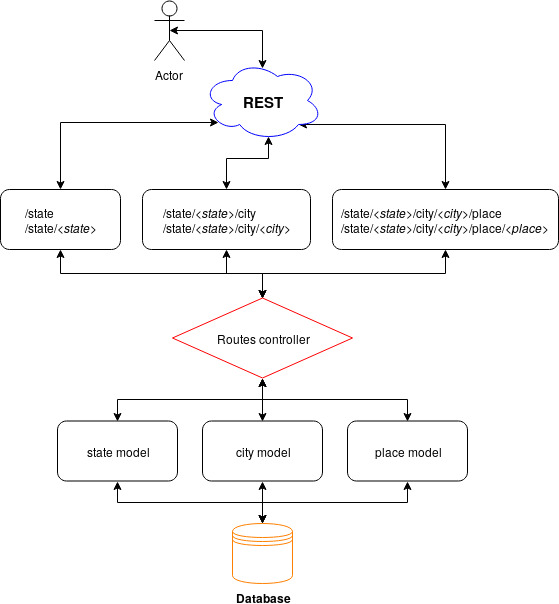
\includegraphics[scale=0.45]{imgs/da_rest.jpg}}
\caption{Arquitetura da API REST.}
\label{fig:arq_rest}
\end{figure}

Na arquitetura REST um chamada para API é realizada através do método \textit{GET} e dos seguintes \textit{endpoints}:

\begin{itemize}
    \item \textbf{/state} \\
    Retorna todos estados brasileiros.
    \item \textbf{/state/\textit{:state}} \\
    Retorna todos estados brasileiros que combinem com \textit{:state}.
    \item \textbf{/state/\textit{:state}/city} \\
    Retorna todas cidade de \textit{:state}.
    \item \textbf{/state/\textit{:state}/city/\textit{:city}} \\
    Retorna todas cidade de \textit{:state} que combinem \textit{:city}.
    \item \textbf{/state/\textit{:state}/city/\textit{:city}/place} \\
    Retorna todos logradouros da cidade \textit{:city} pertencentes ao estado \textit{:state}.
    \item \textbf{/state/\textit{:state}/city/\textit{:city}/place/\textit{:place}} \\
    Retorna todos logradouros que combinem com \textit{:place}, da cidade \textit{:city} pertencente ao estado \textit{:state}.
\end{itemize}

Os campos com prefixo ':' indica onde o texto da requisição é inserido para buscar por semelhança, sendo assim, para consultar todas as cidades do estado da Bahia poderia ser utilizado \textit{/state/\textbf{Bahia}/city} ou \textit{/state/\textbf{ba}/city} para retornar todas cidades (\textit{city}) de estados (\textit{state}) que possuem a subcadeia \textbf{ba} em seu nome. Ressalta-se também que a busca não utiliza \textit{case sensitive}, ou seja, não faz diferença o uso de \textbf{Bahia} ou \textbf{bahia}. A mesma situação acontece para busca de nome de cidades. O caso especial está na busca por \textit{place}, na qual a combinação é comparada com CEP, bairro e logradouro da tabela.

Com todos conceitos informados anteriormente, torna-se simples entender o fluxo apresentado na Figura \ref{fig:arq_rest}. Uma solicitação por \textit{endpoint} é feita na API REST, a mesma aciona o controlador de rotas (\textit{Routes controller}) que indica qual ação deve ser tomada, utilizando o \textit{model} específico para a resposta. O \textit{model}, por sua vez, manipula o banco de dados (\textit{database}), reagindo à ação, e retorna o resultado para o caminho inverso com a resposta da solicitação.

\begin{figure}[htbp]
\centerline{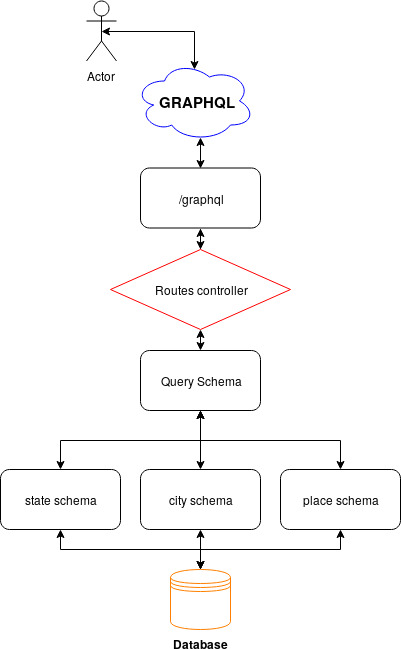
\includegraphics[scale=0.45]{imgs/da_graphql.jpg}}
\caption{Arquitetura da API GraphQL.}
\label{fig:arq_graphql}
\end{figure}

A estrutura e comportamento da aplicação GraphQL é semelhante à REST. A diferença pode ser observada nos \textit{endpoints} e \textit{models}. Na GraphQL, um único \textit{endpoint} é utilizado com requisição por método \textit{POST} e, seus \textit{models} são representados como \textit{schemas}. Outro aspecto, refere-se à adição de mais uma camada de controle (\textit{Query Schema}) que é responsável por intermediar a comunicação do \textit{controller} com os \textit{schemas}. A Figura \ref{fig:req_rg} exemplifica o \textit{endpoint} e corpo de uma requisição para a REST e a GraphQL.

\begin{figure}[htbp]
\centerline{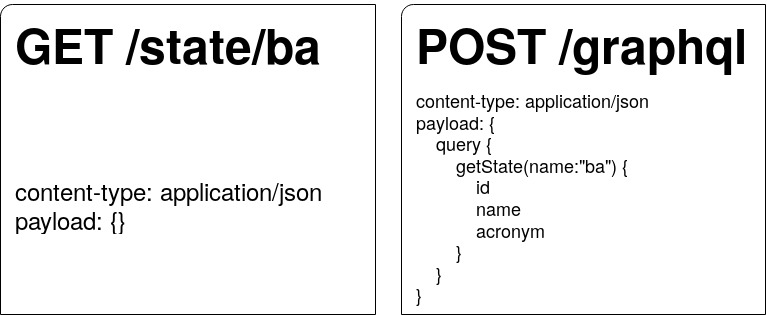
\includegraphics[scale=0.30]{imgs/req_rest_graphql.jpg}}
\caption{Corpo da requisição com REST (esquerda) e GraphQL (direita).}
\label{fig:req_rg}
\end{figure}

De forma resumida, fica perceptível que toda arquitetura foi desenvolvida para fornecer variações de consultas de endereços seguindo um modelo em árvore, no qual a raiz seria os estados (Figura \ref{fig:arvore_req}).

\begin{figure}[htbp]
\centerline{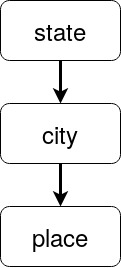
\includegraphics[scale=0.45]{imgs/arvore_req.jpg}}
\caption{Árvore de requisição.}
\label{fig:arvore_req}
\end{figure}

Caso haja necessidade de realizar a requisição sem nenhum filtro, basta fornecer o valor '\%' para o campo de busca, que possibilita o retorno de todos os registros. Devido à limitações físicas, por padrão, existe um tamanho fixo de 10 (dez) registros retornados por requisição, a fim de evitar insucessos durante as consultas. Podem ser utilizados para modificar tal comportamento, o parâmetro \textit{limit} (padrão 10) e também o \textit{page} (padrão 0), respectivamente, o que indica a quantidade de registros máximos por página e o que indica qual página deseja-se obter. A Figura \ref{fig:req_rg_lp} exemplifica a alteração dos parâmetros.

\begin{figure}[htbp]
\centerline{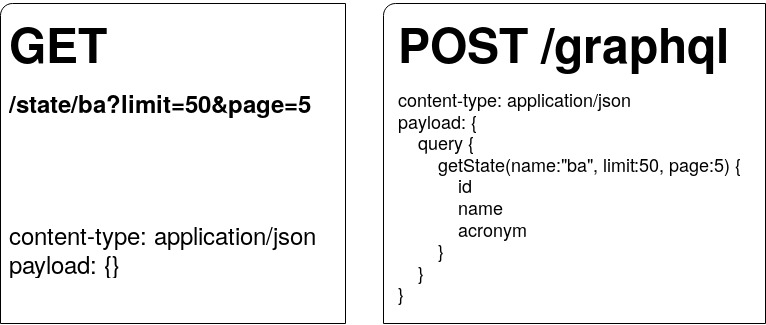
\includegraphics[scale=0.30]{imgs/req_rest_graphql_lp.jpg}}
\caption{Corpo da requisição com REST (esquerda) e GraphQL (direita), parametrizando o tamanho limite da resposta.}
\label{fig:req_rg_lp}
\end{figure}

\begin{figure}[htbp]
\centerline{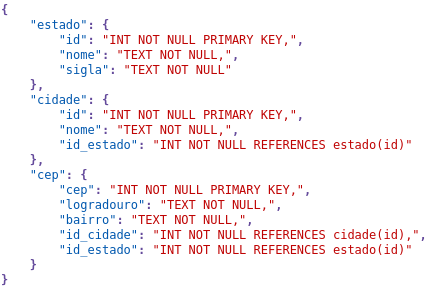
\includegraphics[scale=0.45]{imgs/struct_json.png}}
\caption{Arquivo JSON utilizado para modelagem física.}
\label{fig:struct_json}
\end{figure}

O script de pré-processamento foi responsável pela modelagem física do banco de dados, consultando como será a estrutura através de um arquivo JSON com o \textit{key-value pair = \{atributo: descrição\}} (Figura \ref{fig:struct_json}) e como popular as tabelas modeladas, seguindo os passos:

\begin{enumerate}
    \item \textit{Download} da base de dados do CEP Aberto em formato \textit{.zip}.
    \item Descompactação em uma única pasta de pré-processamento.
    \item Criação da modelagem física no postgres utilizando o arquivo JSON para referência.
    \item Leitura dos arquivos ".txt" descompactados
    \item Limpeza das strings adicionando \textit{scapes}, como exemplo o das aspas.
    \item Inserção das tuplas nas respectivas tabelas.
\end{enumerate}

A Figura \ref{fig:preprocessing} retrata de forma resumida o pré-processamento.

\begin{figure}[htbp]
\centerline{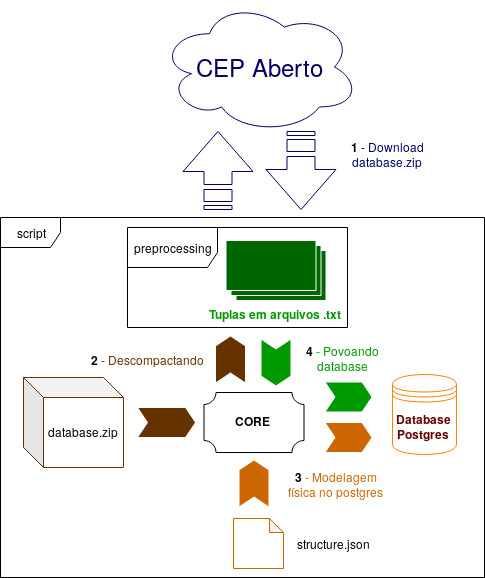
\includegraphics[scale=0.45]{imgs/preprocessing.jpg}}
\caption{Fluxo do pré-processamento de dados.}
\label{fig:preprocessing}
\end{figure}

\section{Análise de desempenho}
\label{sec:analise_desempenho}

\subsection{Pré-processamento}
\label{subsec:pre_processamento}
Inicialmente, foi feita uma tentativa de utilização da base de dados geográficos do OpenStreetMap - OSM \cite{OSM:2019}. A iniciativa deste projeto de mapeamento colaborativo nasceu, visando à criação de um mapa livre e editável do mundo, inspirado por sites como a Wikipédia. Embora seja amplamente divulgado e forneça dados a muitos sites na internet, a aplicações de celular e outros dispositivos, para este trabalho a experiência não foi bem sucedida, em virtude das muitas dificuldades enfrentadas na etapa de pré-processamento dos dados extraídos do OSM.

Importante ressaltar que a maioria das bases geográficas são proprietárias, a exemplo das bases de dados de navegação da Here Technologies \cite{HereTech:2019} e da TomTom \cite{TomTom:2019}. Por serem serviços na nuvem disponibilizados por empresas privadas, são atualizadas constantemente e mais completas que as bases livres, mas obviamente são comercializadas. Por isso, não foram consideradas neste trabalho.

Depois de uma extensa pesquisa, optou-se por utilizar os dados do CEP Aberto \cite{CEPAberto:2019}, que é um projeto que visa prover acesso gratuito e construir, de maneira colaborativa, uma base de dados com os Códigos de Endereçamento Postal - CEP geolocalizados de todo o Brasil. A ideia é que cada indivíduo possa colaborar, melhorando a informação de CEPs que conhece. Mediante registro, qualquer pessoa, gratuitamente, pode ter acesso a API e baixar a base de dados. O CEP Aberto \cite{CEPAberto:2019} possui informação de 980.955 CEPs distribuídos em 10.560 municípios brasileiros.

Extrair os dados corretos da base da plataforma CEP Aberto \cite{CEPAberto:2019} foi fundamental. O seu pré-processamento e sua estruturação foram extremamente importantes para a qualidade das informações e resultados do trabalho.

O CEP Aberto \cite{CEPAberto:2019} disponibiliza todos os endereços brasileiros em arquivos em formato ".txt" separados por estado, cidade e cep, sendo o último particionado em cinco arquivos diferentes. Foram 77 arquivos compactados que totalizaram mais de 600 mil endereços brasileiros.

\subsection{Comparação dos Métodos}

O banco dados foi gerado e executado, utilizando uma instância do PostgreSQL \cite{PostgreSQL:2019} no Docker \cite{docker:2019} em um notebook SIM 5110M Core i3-3110M 2.4GHz com 6GB de memória RAM e SSD de 240GB KINGSTON SUV300S com sistema operacional Pop!\_OS 19.04.

As APIs foram desenvolvidas utilizando a linguagem de programação Python \cite{Python:2019} e o Framework Flask \cite{Flask:2019}. 

Todos os testes de análise comparativa foram realizados localmente e de forma isolada. Primeiramente, utilizando a API REST e posteriormente a GraphQL, ambos os testes com a mesma instância do PostgreSQL \cite{PostgreSQL:2019}.

Conforme mencionado na Subseção \ref{subsec:metricas}, a avaliação foi realizada comparando o \textit{overfetching} e a latência. As requisições foram feitas utilizando os três níveis da árvore de requisição (Figura \ref{fig:arvore_req}), sendo o nível 0, consultas em estados; o nível 1, incluindo cidades e o nível 2, acrescentando os logradouros.

Em cada nível, houve um tamanho de bloco a ser requisitado, variando do menor para o maior, ou seja, no nível 0 (estados), 1 (cidades) e 2 (logradouros) foi possível obter os tamanhos de blocos:

\begin{itemize}
    \item em 0: (id), (id, name), (id, name, acronym);
    \item em 1: (id), (id, idState), (id, idState, name);
    \item em 2 (cep), (cep, idState), (cep, idState, idCity), (cep, idState, idCity, ditrict), (cep, idState, idCity, district, publicPlace);
    \item e também variações de tamanhos mesclando os três níveis, ou seja, utilizado apenas "\textit{name}" do nível 0 e 1, e o "\textit{district}" (bairro) do nível 2.
\end{itemize}

As requisições foram realizadas utilizando os diversos tamanhos de blocos possíveis e a análise ponderou a quantidade de dados úteis e totais retornados pela API GraphQL em comparação a REST. O tempo foi calculado utilizando a biblioteca \textit{timeit} do Python \cite{Python:2019}, sendo destacado pela acurácia. Para cada tamanho de bloco possível foi realizado 100 requisições para o cálculo do tempo médio, e os dados úteis e totais retornados foram mensurados utilizando as próprias informações do \textit{header} (cabeçalho).

\subsection{Resultados}

Os resultados apresentados a seguir foram obtidos com três tamanhos de blocos possíveis (mínimo, médio e máximo) para cada escopo, sendo os três escopos:

\begin{itemize}
    \item Local:
        \begin{itemize}
            \item Mínimo: Obtendo apenas os nomes dos estados.
            \item Médio: Obtendo os nomes e siglas dos estados.
            \item Máximo: Obtendo todas informações dos estados.
        \end{itemize}
    \item Fronteira:
        \begin{itemize}
            \item Mínimo: Obtendo apenas os nomes dos estados e nomes das respectivas cidades.
            \item Médio: Obtendo os nomes dos estados e os nomes e \textit{ids} das respectivas cidades.
            \item Máximo: Obtendo todas informações dos estados e suas cidades.
        \end{itemize}
    \item Global:
        \begin{itemize}
            \item Mínimo: Obtendo as siglas dos estados, nomes das cidades e os CEPs dos logradouros.
            \item Mínimo: Obtendo todas informações dos estados, nomes e \textit{ids} das cidades e os CEPs e barrios dos logradouros.
            \item Máximo: Obtendo todas informações dos logradouros com suas cidades e estados.
        \end{itemize}
\end{itemize}

Para todos os escopo foram definidos os parâmetros de pesquisa com \textit{page} 0 e \textit{limit} de 20.000 registros.

Devido a diversa quantidade de variações do tamanho do bloco, apenas os mecionados anteriormente foram adotados, sendo escolhido dessa forma para melhor distribuição e diferença em relação aos tamanhos e possíveis variações de tempo que poderiam ocorrer.

As requisições forem feitas utilizando um \textit{script} python automatizado com o pacote \textit{requests}. Os tempos foram cálculados considerando apenas a latência das requisições, ou seja, a "chamada" de função GET, em REST, e POST, em GraphQL, do pacote \textit{requests}. Os resultados do script foram armazenados em um arquivo \textit{json} contendo uma lista de "dicionários" com o conjunto de dados em formato \textit{key-value pair}, descritos da seguinte forma:

\begin{itemize}
    \item "scope": O escopo que foi utilizado para requisição (local, border (fronteira), global)
    \item "blockSize": o tamanho do bloco definido para requisição (min, med, max).
    \item "size": o tamanho efetivo do bloco retornado.
    \item "time": um array com os 100 períodos de tempo obtido com o temporizador da requisição.
\end{itemize}

A Figura \ref{fig:estrutura_resultados} exemplifica o corpo do arquivo de resultados.

\begin{figure}[htbp]
\centerline{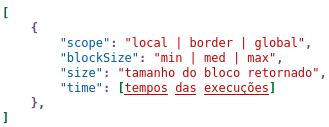
\includegraphics[scale=0.45]{imgs/estrutura_resultados.png}}
\caption{Estrutura do arquivo de resultados.}
\label{fig:estrutura_resultados}
\end{figure}

O cáculo do tamanho de bloco total e útil foi realizado considerando as resposta das requisições GraphQL como sendo sempre de "tamanho útil", e com esse resultado é obtido a proporção de overfetching que o REST possui superior ao GraphQL através da diferença entre ambos. Analisando os resultados obtidos na Tabela \ref{tab:prop_overfetching}, observa-se que o comportamento do REST possui maior overfetching quando são requisitados menores conjuntos de dados das APIs independente do escopo. Ressalta-se também tal comportamento no escopo global, em a requisição solicita todas entidades disponíveis (estados, cidades, cep), havendo uma redução razoável a medida que aprofundamos a árvore de requisição (Figura \ref{fig:arvore_req}).

\begin{table}
\renewcommand{\arraystretch}{1.3}
\caption{Proporção de overfetching em REST superior ao GraphQL.}
\label{tab:prop_overfetching}
\centering
\begin{tabular}{ll|rrr}
    \multirow{2}{*}{Escopo} & \multirow{2}{*}{Tipo} & \multicolumn{2}{c}{Resposta da arquitetura (bytes)} & \multirow{2}{*}{\% ($\approx$)}\\
    && REST & GraphQL & \\
    \hline
    \multirow{3}{*}{local} & min & 1966 & 365 & 81.43\\
    & med & 1966 & 590 & 69.99\\
    & max & 1966 & 705 & 64.14\\
    \multirow{3}{*}{fronteira} & min & 1092575 & 7213 & 99.34\\
    & med & 1092575 & 9789 & 99.10\\
    & max & 1092575 & 13466 & 98.77\\
    \multirow{3}{*}{global} & min & 4232448 & 347057 & 91.8\\
    & med & 4232448 & 906716 & 78.58\\
    & max & 4232448 & 2274673 & 46.26
\end{tabular}
\end{table}

Devido ao ambiente não controlado e compartilhado, algumas discrepâncias de latência surgiram. A Figura \ref{fig:rest_border_scope} exibe o pior caso de outlier encontrado na execução da API REST (escopo de fronteira). Enquanto que na Figura \ref{fig:graphql_global_scope_max} apresenta o pior caso para a arquitetura GraphQL onde o tamanho de bloco foi do tipo máximo.

\begin{figure}[htbp]
\centerline{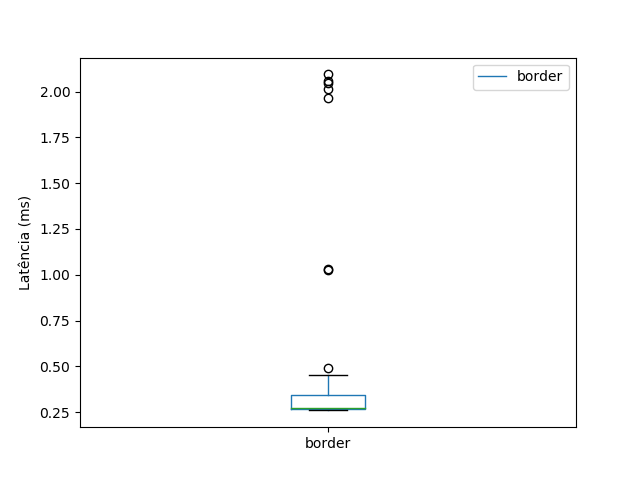
\includegraphics[scale=0.50]{imgs/rest_time/border_rest.png}}
\caption{Outliers do escopo de fronteira para API REST.}
\label{fig:rest_border_scope}
\end{figure}

\begin{figure}[htbp]
\centerline{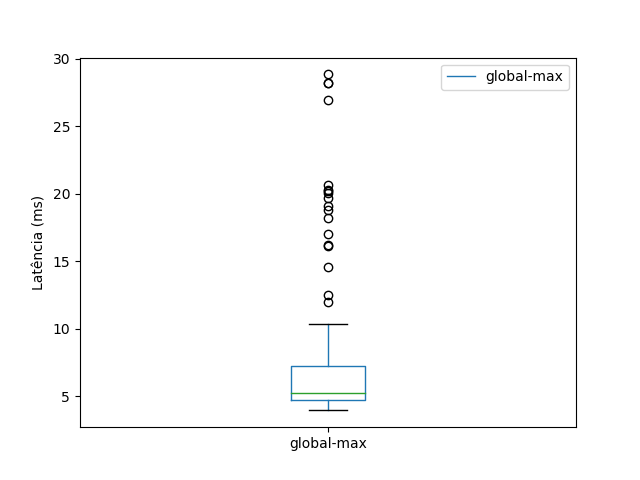
\includegraphics[scale=0.50]{imgs/graphql_time/global_graphql-max.png}}
\caption{Outliers do escopo global e tamanho de bloco do tipo máximo para API GraphQL.}
\label{fig:graphql_global_scope_max}
\end{figure}

Ressalta-se que em todos tamanhos de blocos: mínimo, médio e máximo, a API REST gerou resultados semelhantes.

Os outliers foram tratados utilizando a regra 1,5xIQR (Interquartile range), que informa de que modo os valores médios estão espalhados, utilizando a Equação \ref{eq:iqr}, onde $q_1$ é o primeiro quartíl e $q_3$ é o terceiro quartíl.
\begin{equation}
iqr = q_3 - q_1\label{eq:iqr}
\end{equation}

Desse modo, foi possível obter os resultados de latência conforme apresentados na Tabela \ref{tab:latencia}. É observado que ambas arquiteturas possuem a latência diretamente proporcional a complexidade do escopo. Alguns comportamentos podem ser destacados, como: a similaridade entre as latências de escopo local e de fronteira no GraphQL, possivelmente devido ao corpo da requisição serem equivalentes; e a semelhança entre os resultados obtidos em GraphQL para o mesmo tipo de tamanho (min, med, max), que talvez esteja interligado a estabilidade para acesso ao banco de dados.
 
\begin{table}
\renewcommand{\arraystretch}{1.3}
\caption{Proporção de overfetching em REST superior ao GraphQL.}
\label{tab:latencia}
\centering
\begin{tabular}{ll|rr}
    \multirow{2}{*}{Escopo} & \multirow{2}{*}{Tipo} & \multicolumn{2}{c}{Tempo médio da arquitetura (ms)} \\
    && REST & GraphQL \\
    \hline
    \multirow{3}{*}{local} & min & 0.00699157929033343 & 2.774390276240301 \\
    & med & 0.00699157929033343 & 2.844395469267839 \\
    & max & 0.00699157929033343 & 2.791358945252202 \\
    \multirow{3}{*}{fronteira} & min & 0.30514050403318155 & 2.812832926094339 \\
    & med & 0.30514050403318155 & 2.760971944828525 \\
    & max & 0.30514050403318155 & 2.6593246800774875 \\
    \multirow{3}{*}{global} & min & 3.2016676112147078 & 3.726284877153895 \\
    & med & 3.2016676112147078 & 5.119934367011191 \\
    & max & 3.2016676112147078 & 5.351672762182805
\end{tabular}
\end{table}

\section{Discussão}
\label{sec:discussao}

Este trabalho investigativo projetou, desenvolveu e testou uma API REST e outra API GraphQL, com o intuito de comparar o desempenho de ambas, no tocante à eficiência, especificamente à categoria comportamento em relação ao tempo, latência, e à categoria utilização de recursos, \textit{overfetching}. 

Os resultados da pesquisa têm implicações significativas para a tomada de decisão com relação à arquiteturas de TI que venham a ser implementadas com a linguagem de programação Python e o banco de dados PostgreSQL, bem como acessem endereços em bases de dados georreferenciados.

Diante do exposto, conclui-se que:

\begin{itemize}
    \item Uma implementação confiável do estilo de arquitetura REST em uma API apresentou uma resposta mais rápida do que uma API criada com a tecnologia GraphQL.
    \item Os tamanhos das respostas de uma API GraphQL são consideravelmente menores do que os tamanhos das respostas geradas por uma API que segue as restrições do estilo da arquitetura REST.
    \item Existe algum comportamento interessante em relação a estabilidade da latência no GraphQL, sendo seus resultados muito próximos.
    \item Curiosamente, um caso foi identificado quanto ao \textit{overfetching} em REST nos escopos com tamanho de tipo máximo. Embora as requisições para ambas as arquiteturas estejam solicitando o maior conjunto de dados disponíveis, o REST ainda apresenta, no melhor caso, um \textit{overfetching} de $46.26\%$ superior ao GraphQL, comportamento não identificado mas talvez ligado à duplicidade de informações no corpo da resposta em REST.
\end{itemize}

Alguns desafios e desvantagens a serem considerados nesta abordagem:

\begin{itemize}
    \item Poderiam ser aplicados testes com variações no tamanho do \textit{limit}. Isso aumentaria o conjunto de endereços, englobando não somente o Brasil. Desse modo, seria possível expandir o campo de busca. Embora o \textit{limit} tenha sido definido em 20.000 endereços, a quantidade de estados brasileiros, por exemplo, possuem bem menos que isso.
    \item Necessidade de executar os testes realizados, em ambiente controlado. Na execução local, existe um constante compartilhamento de recursos e muitas vezes processos que são alocados e desconhecidos. Um ambiente controlado seria ideal para realizar o cálculo da latência, por exemplo.
    \item Ressalta-se que, mesmo tendo sido aplicada uma função para reduzir os outliers, ainda pode haver muito ruído nos dados de latência, pelos mesmos motivos destacados no item anterior.
\end{itemize}

A partir deste estudo, trabalhos futuros poderão explorar outros tipos de testes de software. Por exemplo, testes de carga e stress, para comparar como ambas as arquiteturas reagem à requisições constantes sem ociosidade de tempo. Simultaneamente, verificar o uso dos recursos computacionais que cada uma utiliza para dar uma resposta.

\bibliographystyle{IEEEtran}
\bibliography{bibtex}

\end{document}

% \lipsum[1] % filler text
% \begin{table*}
%  \caption{CIFAR-10 Confusion Matrix}
% \label{my-label}
% \begin{tabularx}{\textwidth}{@{}l*{10}{C}c@{}}
% \toprule
% labels     & airplane & automobile & bird & cat & deer & dog & frog & horse & ship & truck & accuracy \\ 
% \midrule
% airplane   & 915      & 4          & 17   & 19  & 3    & 1   & 0    & 2     & 27   & 12    & 91.50\%  \\ 
% automobile & 8        & 934        & 3    & 4   & 0    & 0   & 3    & 0     & 10   & 38    & 93.40\%  \\ 
% bird       & 60       & 1          & 813  & 37  & 19   & 23  & 30   & 10    & 7    & 0     & 81.30\%  \\ 
% cat        & 18       & 1          & 34   & 746 & 25   & 113 & 37   & 18    & 8    & 0     & 74.60\%  \\ 
% deer       & 24       & 1          & 38   & 33  & 809  & 19  & 44   & 29    & 2    & 1     & 80.90\%  \\ 
% \addlinespace
% dog        & 4        & 0          & 37   & 106 & 23   & 792 & 9    & 26    & 2    & 1     & 79.20\%  \\ 
% frog       & 2        & 5          & 19   & 35  & 1    & 20  & 912  & 2     & 3    & 1     & 91.20\%  \\ 
% horse      & 14       & 0          & 26   & 20  & 18   & 28  & 4    & 886   & 3    & 1     & 88.60\%  \\ 
% ship       & 35       & 10         & 3    & 2   & 0    & 2   & 1    & 0     & 936  & 11    & 93.60\%  \\ 
% truck      & 23       & 37         & 4    & 10  & 1    & 2   & 2    & 0     & 15   & 906   & 90.60\%  \\ 
% \bottomrule
% \end{tabularx}
% \end{table*}
% \lipsum[2-15] % more filler text